%!TEX program = xelatex
%!TEX builder = latexmk
% or can be latexmk texify
%!TEX option = 
% -shell-escape -8bit % For minted package
%!TEX root = ...
\documentclass[8pt,a4paper,twocolumn]{article} % titlepage表示标题单独页
\usepackage[noindent]{ctex} % ctex套用英文标题格式 (建议在英文论文混排中文时使用) ,
% ctexcap套用中文格式 (等同于\documentclass{ctexart}) 
% \renewcommand{\figurename}{图}
% \renewcommand{\tablename}{表}
% \renewcommand{\contentsname}{目录}
% \renewcommand\refname{参考文献}
% \renewcommand{\thefigure}{\chinese{figure}} % 将图片计数改为汉字数字
% \renewcommand{\thetable}{\chinese{table}} % 将表格计数改为汉字数字
\usepackage[top=0.75in,bottom=0.75in,left=0.75in,right=0.75in]{geometry} % 页边距设置
% \usepackage{multicol}页面内多行包
\usepackage[CJKbookmarks]{hyperref} % 给pdf文档添加互动式链接和书签
\hypersetup{linktocpage=true}%make the link of the content on the number of page
% \userpackage{wrapfig} % 图文绕排
% \usepackage{xeCJK} % to get my Chinese name
% \setCJKmainfont{SimSun}
% \usepackage[parfill]{parskip} % 增加段间行距
\usepackage{amsmath,amssymb,esint} % 数学公式类宏包;最末为积分符号拓展
\allowdisplaybreaks[0]% 允许多行公式间换页, 用//*表示不允许换页
\numberwithin{equation}{section} % 公式编号包含章节
\usepackage{bm} % 加粗 (用于vector) 
\usepackage{mathrsfs} % mathscr font
% \usepackage{textcomp} % 符号包, 不能用于数学模式, 建议不要和SIunits混用
% \usepackage[squaren]{SIunits} % 科学单位包, 可以用于数学模式
% (为了统一不要和textcomp混用) , squaren选项消除和amssymb的冲突
\usepackage{siunitx} % 淘汰掉上面这个宏包吧, 现在用的是
% \num{123}, \si{kg.m/s^2}, 
% \si{\electronvolt\per\square\clight}, \SI{123}{\micro\metre}
\usepackage{extarrows} % 长箭头, 长等号etc.
\usepackage{graphicx} % 插图宏包
% \usepackage{picinpar} % 图文绕排
\usepackage{array} % 表格宏包
% \usepackage{longtable} % 长表格宏包
\usepackage{multirow} % 多行合并的表格宏包
% \usepackage{booktabs} % 表格线宏包
\usepackage{braket} % 狄拉克符号

% \usepackage[basic,box,gate,oldgate,ic,optics,physics]{circ} % 电路图宏包
% \usepackage[normalem]{ulem} % 下划线, 删除线等宏包, 参数表示不修改\emph{}格式
% \usepackage{mychemistry} % 化学宏包, 包含mhchem和chemfig
% \usepackage[version=3]{mhchem} % 化学宏包, 包含mhchem和chemfig
% \usepackage[symbol]{footmisc} % 脚注拓展, 选项表示用符号做脚注记号
% \usepackage{listings} % 代码段宏包
% \lstset{numbers=left,frame=shadowbox,%
% basicstyle=\ttfamily, commentstyle=\fontseries{lc}\selectfont\itshape, %
% columns=fullflexible, breaklines=true, escapeinside={(*@}{@*)}}
% \usepackage{minted} % 具有 Python 支持的代码宏包

% \renewcommand*{\vec}[1]{\bm{#1}} % 矢量的格式, 这里是加粗
\newcommand{\dif}{\,\mathrm d}
\newcommand\mi{\mathrm{i}}
\newcommand\e{\mathrm{e}} % 定义数学模式中常用的正体字符
\newcommand\Y{\mathrm{Y}}
\newcommand\cc{\mathrm{c.c.}}
\DeclareMathOperator{\Imag}{Im}
\bibliographystyle{unsrt}

\begin{document}\small
	\title{Circuit Quantum Electrodynamics}
	\author{Wentao Jiang}
	\date{}
	\maketitle
	\tableofcontents
	\section{Introduction} % (fold)
	\label{sec:introduction}
		Requirements of a quantum computer:
		\begin{enumerate}
    		\setlength{\itemsep}{1pt}
    		\setlength{\parsep}{1pt}
    		\setlength{\parskip}{1pt}
			\item isolated from sources of noise
			\item strongly coupled to each other
			\item refer to \cite{DiVincenzo2000} for more and detailed requirements
		\end{enumerate}
		Cavity QED system: an atom modeled as a two-level system coupled to a harmonic oscillator, whose excitations are photons.

		cQED-like systems: 
		\begin{itemize}
			\item alkali atoms above an optical cavity formed by two mirrors, readout by transmission of a laser through the cavity
			\item Rydberg atoms with 3-D microwave cavities, require cooling to $\sim$1K, use atoms to probe the cavity photons by selective ionization
		\end{itemize}

		\subsection{Quantum Circuits} % (fold)
		\label{sub:quantum_circuits}
			the only known dissipationless non-linear circuit element

			High frequencies (GHz) LC circuit at low temperatures (<100mK) will have resolvable energy levels corresponding to microwave photons. However, its harmonicity makes it impossible to observe the discrete nature of these photons.

			Josephson junction, cooper pair box (CPB): enhance nonlinearity

			Atoms: quantum purity for $10^{14}$ periods, hard to tune

			Artificial atoms (quantum dots, CPB): more tunable, more decoherence
		% subsection quantum_circuits (end)

		\subsection{Circuit Quantum Electrodynamics} % (fold)
		\label{sub:circuit_quantum_electrodynamics}
			Superconductive circuits $\Longleftrightarrow $ artificial atoms

			Key to cQED readout: use 1-D coplanar waveguide (CPW) resonator as a cavity

			Benefits:
			\begin{itemize}
				\item travel length of MW photon in CPW: 10km
				\item stronger coupling (10000 times larger than ordinary alkali atom, 10 times larger than Rydberg atom)
				\item 1-D transmission line cavity increasing the energy density by $10^6$ over 3-D MW cavities, further increase dipole coupling by 1000
			\end{itemize}

		% subsection circuit_quantum_electrodynamics (end)

	% section introduction (end)

	\section{Cavity Quantum Electrodynamics} % (fold)
	\label{sec:cavity_quantum_electrodynamics}
		\begin{figure}[!h]
			\centering
			%width can be changed
			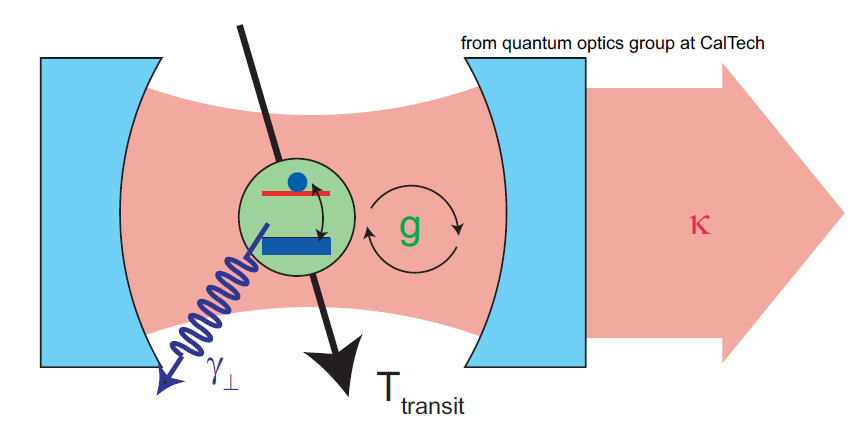
\includegraphics[width=2in]{cavityQED.png}
			\caption{A two level atom interacts with the field inside of a high finesse cavity. \cite{Schuster2007}}
			\label{pic:cavityQED}
		\end{figure}
		\begin{figure}[!h]
			\centering
			%width can be changed
			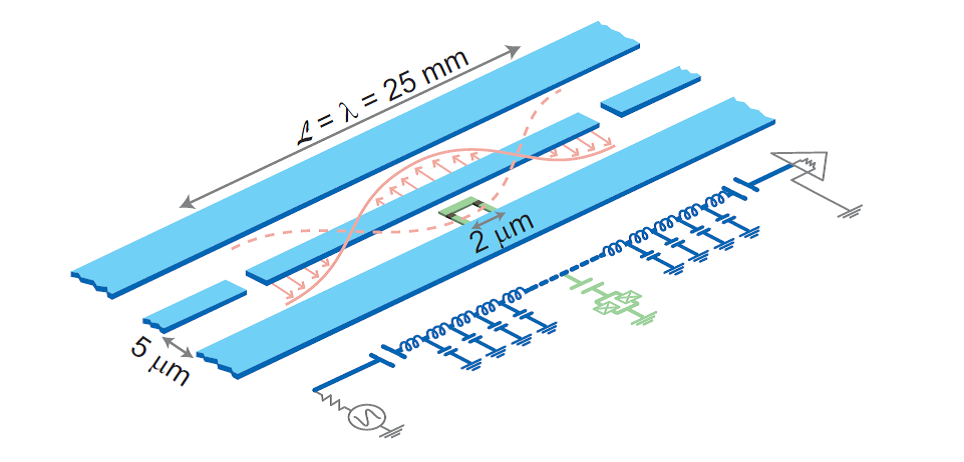
\includegraphics[width=3in]{cQEDwithSuCondQubit.png}
			\caption{Schematic representation of cavity QED with superconducting circuits. \cite{Schuster2007}}
			\label{pic:cQEDwithSuCondQubit}
		\end{figure}
		Jaynes-Cummings Hamiltonian:
		\begin{equation}
			H_{\text{JC}} = \hbar \omega_r (a^{\dagger}a+1/2)+ \hbar \frac{\omega_a}{2} \sigma_z + \hbar g ( a^{\dagger} \sigma^- + a \sigma^+ )
		\end{equation}

		$g $: coupling rate

		$\kappa $: photon decay rate

		$ Q=\omega_r/\kappa $: quality factor

		$ \gamma_{\perp} $: atom decay rate

		$T_{\text{transit}}$: atom transit time before leaving cavity

		When the atom is resonant with the cavity, the two system can freely exchange energy. When many oscillations can be completed before the atom decays, it's called the \textbf{strong coupling} limit: $g>\gamma,\kappa,1/T_{\text{transit}} $.

		\begin{figure}[!h]
			\centering
			%width can be changed
			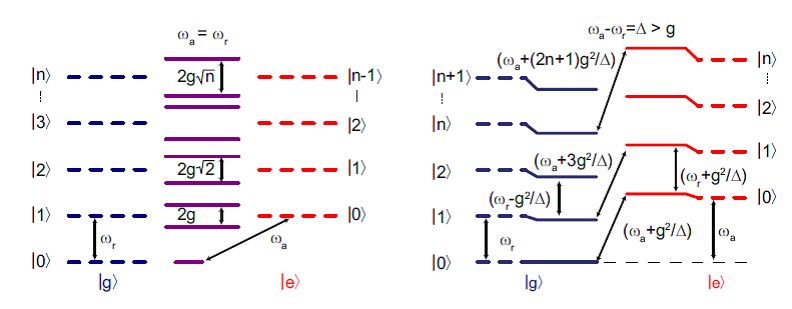
\includegraphics[width=3in]{JClevels.png}
			\caption{Energy level diagram of the J-C Hamiltonian. \cite{Schuster2007}}
			\label{pic:JClevels}
		\end{figure}

		Eigenstates: $ \ket{\psi_{\pm} } = ( \ket g \ket n \pm \ket e \ket{n-1} )/\sqrt 2 $, whose energies split by $2g\sqrt n$, i.e., energy levels are anharmonic even for single photon in the strong coupling limit.

		Because excitations are equally shared between atoms and the cavity, they decay at $\Gamma_{\text{eff} }=(\gamma_{\perp}+\kappa)/2 $

		Purcell effect(?)

		\subsection{Dispersive Limit} % (fold)
		\label{sub:dispersive_limit}
			Resonant limit: $\Delta=\omega_a- \omega_r \ll g $\\
			Dispersive limit: $\Delta\gg g$\\
			Using perturbation to the interaction part and expand in powers of $g/\Delta $ to second order:
			\begin{equation}
				H\approx \hbar \left( \omega_r +\frac{g^2}{\Delta} \sigma_z \right) (a^{\dagger}a+1/2)+\hbar \omega_a \sigma_z /2
			\end{equation}
			The interaction is through the dispersive shift term proportional to $g^2/\Delta$, which commutes with the rest of the Hamiltonian, conserves both the photon number and the atom state.

			Result: the effective frequency of the cavity $ \omega_r'=\omega_r\pm g^2/\Delta $ depends on the state of the atom.

			Rewrite the Hamiltonian to
			\begin{equation}
				H\approx \hbar(a^{\dagger}a+1/2) +\frac{\hbar}{2} \left( \omega_a +\frac{2g^2}{\Delta}a^{\dagger}a + \frac{g^2}{\Delta}\right) \sigma_z /2
			\end{equation}

			Result: the interaction gives the atom frequency a ``light'' shift consisting of a photon number-dependent ``Stark'' shift $ 2ng^2/\Delta $ and vacuum noise induced ``Lamb'' shift $g^2/\Delta $

			Accurate general solution:
			\begin{align}
				&E_{\pm,n}=\hbar \omega_r\pm \frac{\hbar}{2} \sqrt{4ng^2+\Delta^2}\\
				&E_{g,0}=-\frac{\hbar \Delta}{2}
			\end{align}
			where $n$ is the total number of excitations, \textbf{not} the number of photons and $\pm$ refer to the higher energy or lower energy state in the $n$ excitation manifold, \textbf{not} the atom state.

			\begin{figure}[!h]
				\centering
				%width can be changed
				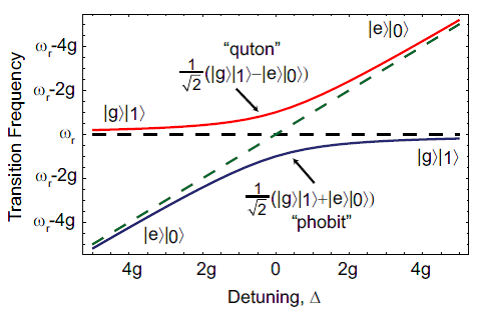
\includegraphics[width=3in]{avoidedCross.png}
				\caption{The avoided crossing in the transition frequency. \cite{Schuster2007}}
				\label{pic:avoidedCross}
			\end{figure}

			Eigenstates:
			\begin{align}
				& \ket{-,n} = \cos \theta_n \ket{g,n} -\sin \theta_n \ket{e,n-1}\\
				& \ket{+,n} = \sin \theta_n \ket{g,n} + \cos \theta_n \ket{e,n-1}\\
				& \theta_n = \frac{1}{2} \arctan \left( \frac{2g\sqrt n}{\Delta} \right)
			\end{align}

			When dispersive limit is reached:
			\begin{align}
				& \ket{-,n} =  \ket{g,n} -\frac{g\sqrt n}{\Delta}  \ket{e,n-1}\\
				& \ket{+,n} = \frac{g\sqrt n}{\Delta}  \ket{g,n} +   \ket{e,n-1}
			\end{align}
			i.e., qubit states have some photon component, which can be used to create an ``entanglement'' bus when multiple qubits are strongly coupled to the same cavity with overlapping photonic part of their wavefunctions.

			Instead of $\Gamma_{\text{eff} }=(\gamma_{\perp}+\kappa)/2 $ as in resonant limit, the qubit has some probability to decay as a photon at a rate $ \gamma_{\kappa} $, because it has a photonic aspect, and vice versa photons can be emitted by the qubit into non-radiative modes at a rate $\kappa_{\gamma} $:
			\begin{align}
				&\gamma_{\kappa}\approx \left( \frac{g}{\Delta} \right)^2 \kappa\\
				&\kappa_{\gamma}\approx \left( \frac{g}{\Delta} \right)^2 \gamma
			\end{align}

			The non-radiative ssource of decay $\gamma_{\perp}$ will begin to dominate before the limit set by suppressed radiative decay.

		% subsection dispersive_limit (end)

		\subsection{Strong Dispersive Interactions} % (fold)
		\label{sub:strong_dispersive_interactions}
			Dispersive regime: $\Delta\gg g$\\
			Strong dispersive regime: $\Delta\gg g$, $\chi = g^2/\Delta > \gamma, \kappa$\\
			i.e., the qubit spectrum resolves into individual photon number peaks, Cavity shift is also larger than cavity linewidth.

			For measuring the state of a single atom using the cavity, one can use many photons to realize it for $\chi<\kappa$. For single photon precision, dispersive strong coupling is required.

			\begin{figure}[!h]
				\centering
				%width can be changed
				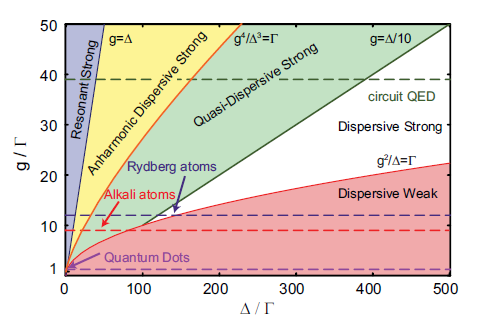
\includegraphics[width=3in]{cQEDphase.png}
				\caption{A phase diagram for cavity QED, described by the atom-photon coupling strength $g$ and the detuning $\Delta$, normalized to the rates of decay $\Gamma = \max[ \gamma,\kappa,1/T ]. $\cite{Schuster2007}}
				\label{pic:cQEDphase}
			\end{figure}

			\begin{figure}[!h]
				\centering
				%width can be changed
				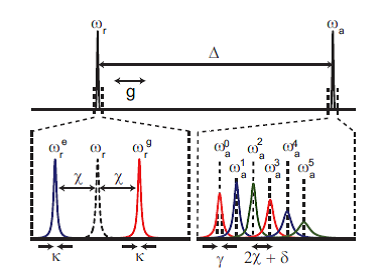
\includegraphics[width=3in]{spectrumInSDlimit.png}
				\caption{Spectrum of coupled cavity and atom system in strong dispersive limit. \cite{Schuster2007}}
				\label{pic:spectrumInSDlimit}
			\end{figure}

			If $\chi>\gamma$ is reached, the atom is shifted by more than a linewidth for each photon, making it possible to measure the exact photon number distribution. A CNOT gate can also be realized if the qubit is made only to respond when a single photon is present.





		% subsection strong_dispersive_interactions (end)


	% section cavity_quantum_electrodynamics (end)

	\section{Cavity QED with Superconducting Circuits} % (fold)
	\label{sec:cavity_qed_with_superconducting_circuits}
		\subsection{The Parallel LCR Oscillator} % (fold)
		\label{sub:the_lcr_oscillator}
			Equation of motion:
			\begin{equation}
				\frac{d^2 q}{dt^2}-\frac{1}{RC}\frac{dq}{dt}+\frac{q}{LC}=0
			\end{equation}
			Solution:
			\begin{equation}
				q(t)=q_0\exp\left[ i(\omega_0 +i \frac{\kappa}{2})t+\phi \right]
			\end{equation}
			where charge oscillation frequency $\omega_0=1/\sqrt{RC} $ and decay rate $ \kappa=2/RC $.\\
			Impedance:
			\begin{equation}
			\label{eqt:LCR_Impedance}
				Z_{LCR}(\omega)=\left( j \omega C+\frac{1}{j \omega L}+\frac{1}{R} \right)^{-1}=\frac{R}{1+2jQ \delta \omega/\omega_0}
			\end{equation}
			where the quality factor $Q=\omega_0 RC $

		% subsection the_lcr_oscillator (end)
		\subsection{Transmission Line as Series of LC Circuits} % (fold)
		\label{sub:transmission_line_as_series_of_lc_circuits}
			
			\begin{figure}[!h]
				\centering
				%width can be changed
				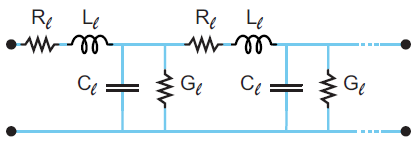
\includegraphics[width=2in]{transmissionLine.png}
				\label{pic:transmissionLine}
			\end{figure}
			Impedance of one small section:
			\begin{equation}
				Z_0=\sqrt{\frac{ R_l +j \omega L_l }{G_l + j \omega C_l}}
			\end{equation}
			Small loss: $ Z_0=\sqrt{L_l/C_l} $\\
			Propagation coefficient: $ \gamma=\sqrt{( R_l +j \omega L_l )(G_l + j \omega C_l)} $\\
			$ \beta=\text{Im} \gamma $ describes the phase, for given frequency, it defines a phase velocity $v=\omega/\beta$\\
			The attenuation $\alpha=\text{Re} \gamma \approx R_l/Z_0+G_l Z_0 $\\
			Effective input impedance of an arbituary load $ Z_l $:
			\begin{equation}
				Z_{\text{in}}=Z_0 \frac{Z_L+Z_0 \tanh \gamma l}{Z_0+Z_L\tanh \gamma l}
			\end{equation}
			where $l$ is the length.

			For termination with high impedances (open/near open), there will be \textbf{two types of resonance}:
			\begin{itemize}
				\item high impedance resonance with $ l=n \lambda/2=\pi v/\omega_0 $
				\item high admittance resonance with $ l=(2n+1)\lambda/4 $
			\end{itemize}
			For the first case:
			\begin{equation}
				Z_{\text{in}}^{\text{open}}=Z_0 \frac{1+j\tan \beta l\tanh \alpha l}{\tanh \alpha l+j\tan \beta l}
			\end{equation}
			For $ \alpha \rightarrow 0 $, i.e., lossless, $ Z_{\text{in}}^{\text{open}} \rightarrow -j\cot \beta l $, which has poles when $ \beta l\approx (n+1)\pi $, expanding for small $ \delta \omega_n $:
			\begin{gather}
				\beta l=(\omega/v)(\pi v/\omega_{\lambda/2})=\pi(n \omega_{\lambda/2} + \delta \omega_n)/\omega_{\lambda/2}\\
				Z_{\text{in}}^{\text{open}}=\frac{Z_0/\alpha l}{1+2j \left( \frac{n \pi}{2 \alpha l} \right) \left( \frac{\delta \omega_n}{n \omega_{\lambda/2}} \right) }
			\end{gather}
			Comparing with eqt \ref{eqt:LCR_Impedance} gives:
			\begin{align}
				&\omega_n = n \omega_{\lambda/2}\\
				&Q_n=R_n /Z_{\text{cn}}=\frac{n \pi}{2 \alpha l}\\
				&R_n = Z_0/ \alpha l = R_l l\\
				&C_n = \frac{Q}{\omega_n R}=\frac{\pi}{2Z_0 \omega_{\lambda/2}}=\frac{1}{2}C_l l\\
				&L_n=\frac{1}{\omega_n^2C}=\frac{2Z_0}{\pi n^2 \omega_{\lambda/2}}=\frac{2}{n^2 \pi^2}L_ll\\
				&Z_{\text{cn}}=\sqrt{L_n/C_n}=\frac{2Z_0}{n \pi}
			\end{align}
			\begin{figure}[!h]
				\centering
				%width can be changed
				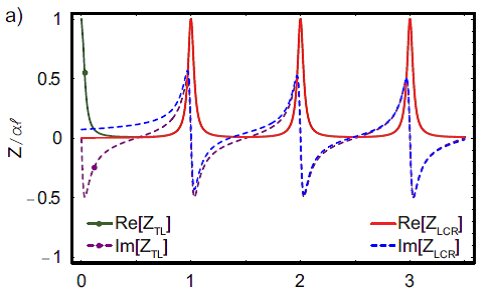
\includegraphics[width=2in]{LCRapprox.png}
				\caption{Real and imaginary parts of the impedance of resonator formed terminating a transmission line with an open-circuit and model of LCR resonators. \cite{Schuster2007}}
				\label{pic:LCRapprox}
			\end{figure}
		% subsection transmission_line_as_series_of_lc_circuits (end)

		\subsection{Coupled LCR Resonator and Transmission Line Resonator} % (fold)
		\label{sub:coupled_lcr_resonator}
			\begin{figure}[!h]
				\centering
				%width can be changed
				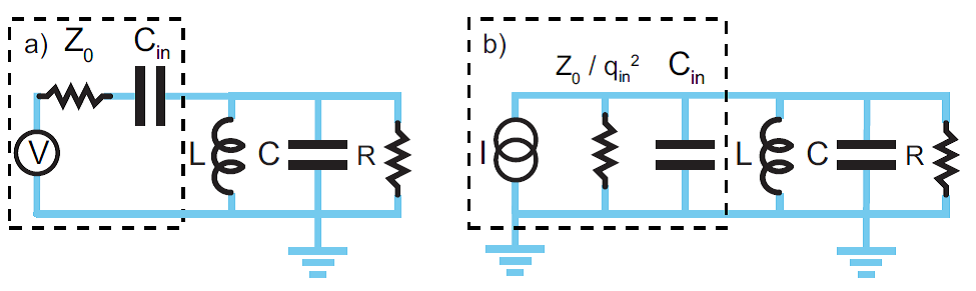
\includegraphics[width=3in]{coupledLCR.png}
				\caption{The capacitive coupling (a) to an environment of impedance Z0 through a capacitor. (b) The transformed input impedance seen by the oscillator. \cite{Schuster2007}}
				\label{pic:coupledLCR}
			\end{figure}
			The effect of the coupling is to add an effective capacitance $ C_{\text{in}} $ and an effective parallel resistance $ Z_0/q_{\text{in}}^2 $, where $ q_{\text{in}}=\omega C_{\text{in}} Z_0 $

			If the internal resistance is negligible:
			\begin{equation}
				Q_{\text{ext}}=\frac{1}{q_{\text{in}}}\frac{Z_0}{Z_{\text{cn}}}\approx \frac{n \pi}{2q_{\text{in}}^2}
			\end{equation}
			If internal resistance is significant compared to the load:
			\begin{equation}
				\frac{1}{Q_L}=\frac{1}{Q_{\text{ext}}}+\frac{1}{Q_{\text{int}}}
			\end{equation}

			In practice it is more convenient to use transmission of a two sided cavity where only the signal is present. If internal losses are negligible and $ Q\gg 1 $:
			\begin{equation}
				S_{21}=\frac{T_0}{1-j \frac{\delta \omega_n}{(\kappa_{\text{in}}+\kappa_{\text{out}})/2}}
			\end{equation}
			where
			\begin{align}
				&\kappa_{\text{in/out}}=\left( \frac{2}{\pi}  \right)q_{\text{in/out}}^2 \omega_n\\
				&T_0 = \frac{\sqrt{\kappa_{\text{in}}\kappa_{\text{out}}}}{(\kappa_{\text{in}}+\kappa_{\text{out}})/2}\\
				&\omega_n = n \omega_{\lambda/2} (1- (q_{\text{in}}+q_{\text{out}}))
			\end{align}
			and reflection:
			\begin{equation}
				S_{11}=\frac{\kappa_{\text{in}}}{\frac{\kappa_{\text{in}}+\kappa_{\text{in}}}{2}-j \delta \omega_n}-1
			\end{equation}
			Transmission phase shift:
			\begin{equation}
				\phi=\arctan\left( \frac{\delta \omega}{\kappa/2} \right)
			\end{equation}
			e.g., $ \phi=\pm\arctan\left( 2g^2/\kappa \Delta \right) $ in strong dispersive interaction\cite{SchusterEtal2005}.
		% subsection coupled_lcr_resonator (end)

		\subsection{Intrinsic Resonator loss} % (fold)
		\label{sub:intrinsic_resonator_loss}
			\begin{itemize}
				\item Resistive Losses: ideally increase exponentially in $ T_c/T $
				\item Dielectric Losses: $ Q_{\text{diel}} =\frac{1}{\tan \delta}$, where $ \tan \delta=-\epsilon_{\text{im}}/\epsilon_{\text{re}} $
				\item Radiative Losses: $Q_{\text{rad}}\approx 3.5 \left( \frac{l}{b} \right)^2$\\
				For experimental parameters: $ l\approx 2.5 $cm, $ b\approx 20 \mu $m, giving $ Q_{\text{rad}}\approx 5\times 10^6 $
			\end{itemize}
			For an approximate overall Q:
			\begin{itemize}
				\item $Q\sim 1500$ in \cite{LarsenEtal2015}
				\item $ Q\approx 10^4 $ in \cite{SchusterEtal2005}
			\end{itemize}
		% subsection intrinsic_resonator_loss (end)

		\subsection{Cooper Pair Box} % (fold)
		\label{sub:cooper_pair_box}
			\begin{figure}[!h]
				\centering
				%width can be changed
				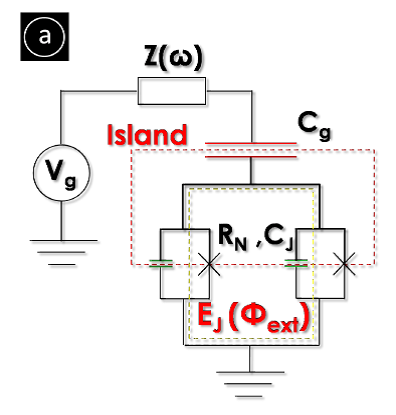
\includegraphics[width=2in]{CPB.png}
				\caption{The circuit diagram of the single Cooper Pair Box.\cite{Krantz2010} }
				\label{pic:CPB}
			\end{figure}
			\begin{figure}[!h]
				\centering
				%width can be changed
				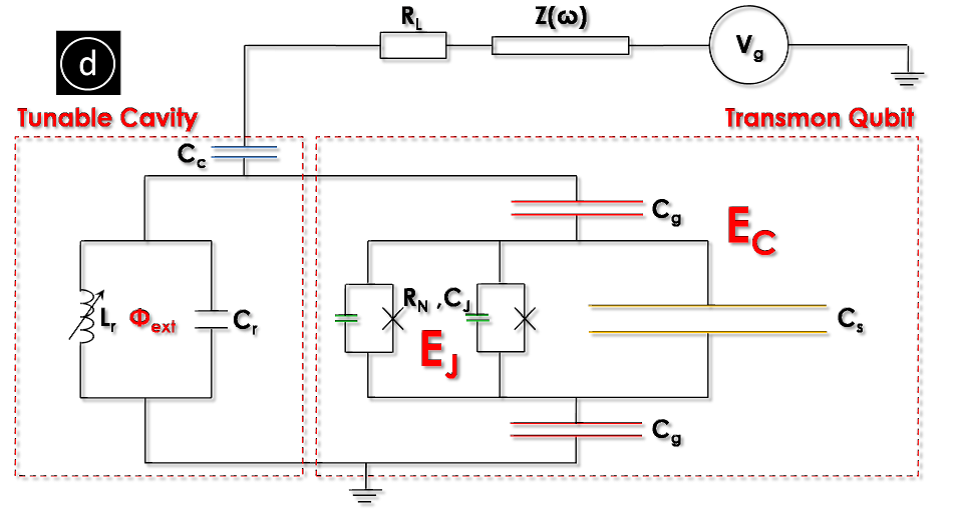
\includegraphics[width=3in]{transmon.png}
				\caption{A transmon coupled to a tunable cavity resonator.\cite{Krantz2010} }
				\label{pic:transmon}
			\end{figure}

			Josephson energy: $ E_J=\frac{R_Q \Delta}{2R_N} $

			Coulomb energy: $E_C=\frac{e^2}{2 C_{\Sigma}}  $\\
			where $ R_Q = h/4e^2 $ is the quantum state resistance, $R_N$ is the normal state resistance, $\Delta$ is the superconducting energy gap. $ C_{\Sigma}=C_g+C_J(+C_s\text{ for transmon}) $ is the total capacitance between the island and its environment.

			$ E_J $ is tunable by an external $B$ field:
			\begin{equation}
				E_J=E_J^{\text{max}}\left| \cos \left( \frac{\pi \Phi_{\text{ext}}}{\Phi_0} \right) \right|
			\end{equation}
			where $\Phi_0=h/2e $ is the flux quantum.

			The Hamiltonian\footnote{$n_g$ is denoted by $n_g/2$ in old literatures (\cite{Schuster2007},\cite{SchusterEtal2005}), here the notation follows \cite{Koch2007} and \cite{Krantz2010}. }:\\
			in charge basis:
			\begin{equation}
				H=4E_C \sum (\hat{n}-n_g)^2 \ket n \bra n -\frac{E_J}{2}\sum[ \ket{n+1}\bra n+ \ket n \bra{n+1} ]
			\end{equation}
			in phase basis:
			\begin{equation}
				H=4E_C(i\frac{d}{d \phi} -n_g)^2-E_J \cos \phi
			\end{equation}
			connected by
			\begin{gather}
				\ket \theta = \sum e^{i \theta n}\ket n\\
				\ket n = \int d \theta e^{-i \theta n}\ket \theta
			\end{gather}
			Energy levels:
			\begin{figure}[!h]
				\centering
				%width can be changed
				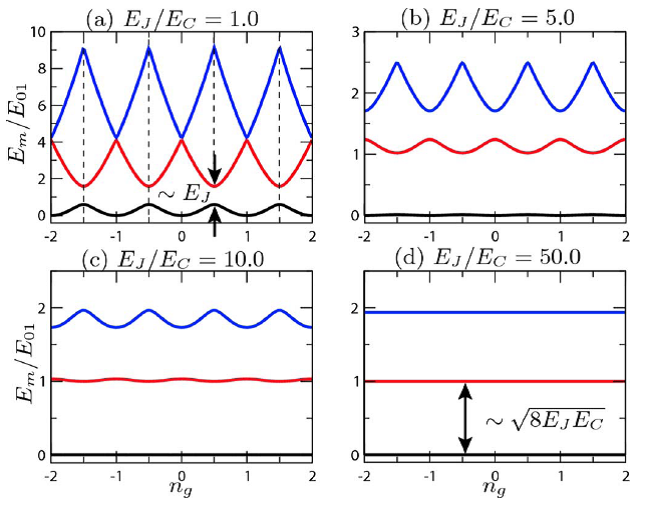
\includegraphics[width=3in]{transmonEnLevel.png}
				\caption{Eigenenergies $E_m$ as a function of the effective offset charge $n_g$ for different $E_J/E_C$ ratios.\cite{Koch2007}}
				\label{pic:transmonEnLevel}
			\end{figure}

			Plasma frequency: $ v_p=\sqrt{8E_JE_C}/h $

		% subsection cooper_pair_box (end)


	% section cavity_qed_with_superconducting_circuits (end)

	\bibliography{CQED}
\end{document}